
\documentclass{report} 

\usepackage{amsmath} % \usepackage is a command that allows you to add functionality to your LaTeX code
\usepackage{graphfig, subfig}
\usepackage{graphicx}
\usepackage{hyperref}
\usepackage{textcase}

\usepackage{geometry}
\geometry{
a4paper,
 total={170mm,257mm},
 left=20mm,
 top=20mm,
}


\usepackage{caption}
\captionsetup{labelformat=empty,textfont=sl}

\usepackage[Glenn]{fncychap}
\title{Storytelling} % Sets article title
\author{Emmanuele Virginio Coppola, Muriel Rossi, Alessandro Marigliano} % Sets authors name

\date{17/07/2022}
\begin{document} % All begin commands must be paired with an end command somewhere 
    \begin{titlepage}
    % Suppresses headers and footers on the title page

	\centering % Centre everything on the title page
	
	\scshape % Use small caps for all text on the title page
	
	\vspace*{\baselineskip} % White space at the top of the page
	
	%------------------------------------------------
	%	Title
	%------------------------------------------------
	
	\rule{\textwidth}{1.6pt}\vspace*{-\baselineskip}\vspace*{2pt} % Thick horizontal rule
	\rule{\textwidth}{0.4pt} % Thin horizontal rule
	
	\vspace{0.75\baselineskip} % Whitespace above the title
	
	{\LARGE SPAMDETECTOR} % Title
	
	\vspace{0.75\baselineskip} % Whitespace below the title
	
	\rule{\textwidth}{0.4pt}\vspace*{-\baselineskip}\vspace{3.2pt} % Thin horizontal rule
	\rule{\textwidth}{1.6pt} % Thick horizontal rule
	
	\vspace{2\baselineskip} % Whitespace after the title block
	
	%------------------------------------------------
	%	Subtitle
	%------------------------------------------------
	
	Un'agente intelligente per la classificazione di commenti spam % Subtitle or further description
	
	\vspace*{3\baselineskip} % Whitespace under the subtitle
	
	%------------------------------------------------
	%	Editor(s)
	%------------------------------------------------
	Professore di Riferimento\\
	
	{\LARGE Fabio Palomba\\}
	
	\vspace{0.5\baselineskip}
	
	Edited By
	
	\vspace{0.5\baselineskip} % Whitespace before the editors
	
	{\scshape\large Coppola Emmanuele Virginio \\ Marigliano Alessandro \\ Rossi Muriel \\} % Editor list
	
	\vspace{0.5\baselineskip} % Whitespace below the editor list
	
	\textit{Università degli studi di Salerno \\ Fisciano} % Editor affiliation
	
	
	\vfill % Whitespace between editor names and publisher logo
	
	{\large Link ai progetti\\}
	\textit{ \href{https://github.com/E-M-A-A/Storytelling}{https://github.com/E-M-A-A/Storytelling}\\
	\href{https://github.com/E-M-A-A/SpamDetectorDev}{https://github.com/E-M-A-A/SpamDetectorDev}
	}
	
	%------------------------------------------------
	%	Publisher
	%------------------------------------------------
	
	%\plogo % Publisher logo
	
	%\vspace{0.3\baselineskip} % Whitespace under the publisher logo
	
	\vspace{0.5\baselineskip}
	
	2022 % Publication year
	
	%{\large publisher} % Publisher

\end{titlepage}
    \tableofcontents
    \chapter{Introduzione} % creates a chapter
    
    La pubblicità invasiva si rivela essere sempre maggiormente un problema asfissiante all'interno del mondo dei socialnetwork. Nonostante siano state sviluppate diverse tecniche
    allo scopo di domare questa piaga, alcune inserzioni riescono tuttavia a sfuggirne, intasando interfacce dedicate all'informazione ed 
    all'intrattenimento, che subiscono così una svalutazione, venendo "soffocate".
    \newline

    \textbf{Legge di Reed: il valore di una rete sociale è direttamente proporzionale ad una funzione esponenziale in N:}
    \begin{equation} % Creates an equation environment and is compiled as math
        V=a*N+b*N^2 + c*2^n
    \end{equation}
    

    La legge sopra citata, descrive come il valore di una rete, formata da interazioni ed intrecci, cresca esponenzialmente con la dimensione di quest'ultima. (1.1).
    In particolare, nel caso di Internet, si osserva come il suo valore tenda a crescere in modo esponenziale se associato a gruppi con interessi
     comuni, che condividono idee, interessi ed obiettivi.
    Da questo se ne deduce come invece, avvisi pubblicitari, spam ed altra "informazione spazzatura", possano far decadere il valore di una rete.
    
    Questo progetto si prefigge lo scopo di manutenere una piattaforma libera dal bombardamento pubblicitario e dare modo all'utenza di potersi esprimere liberamente
    all'interno di questa, distaccandosi dall'ansia e dalla continua distrazione provocata dal chiasso delle inserzioni.
    
    \chapter{Descrizione dell'agente}
    Allo scopo di realizzare questo progetto, è stato introdotto un agente intelligente, sarà lui ad occuparsi della supervisione della piattaforma, indagando fra i 
    commenti relativi alle varie pubblicazioni.
    \section{Obiettivi}
    L'obiettivo dell'agente sarà quello di effettuare un'analisi giornaliera dei commenti relativi ad ogni pubblicazione effettuata dagli utenti della piattaforma.
    Il testo dei vari commenti verrà preso in analisi e, dopo essere stato adeguatamente "pulito", verrà sottoposto all'agente, che sarà in grado di riconoscere se il 
    testo è conforme alle norme della piattaforma (ovvero se non è sospettato come spam). \newline
    In caso negativo, l'autore del commento verrà segnalato alla piattaforma, che provvederà ad eliminarlo da quest'ultima, assieme a tutto il materiale da lui pubblicato.

    \section{Specifiche PEAS}
    Le specifiche PEAS rappresentano diverse proprietà tramite cui è possibile descrivere l'agente. \newline

    \begin{itemize}
        \item 
        {\bfseries P = Performance.} 
        L'agente verrà valutato in base alla percentuale di commenti spam categorizzati correttamente.
        \item 
        {\bfseries E = Environment.} L'agente nel caso in questione lavorerà su query di commenti relativi ai post pubblicati sul Social Network, 
        navigando fra i commenti degli utenti.\newline
        Nello specifico l'ambiente sarà:
            \begin{itemize}
                \item {\bfseries Completamente Osservabile}, in ogni momento l'agente ha completa conoscenza
                dell'ambiente in cui lavora, ovvero la collezione di commenti;
                \item {\bfseries Deterministico}, l'ambiente verrà modificato in base alla decisione dell'agente, 
                ovvero verranno rimossi gli utenti che l'agente deciderà di segnalare;
                \item {\bfseries Episodico}, l'agente viene attivato ad intervalli temporali di 24h. La scelta che compirà l'agente in un singolo episodio dipenderà dall'episodio stesso;
                \item {\bfseries Statico}, mentre analizza la query di commenti, l'ambiente rimane invariato;
                \item {\bfseries Discreto}, l'ambiente fornisce un insieme di parole finite per ogni commento. L'agente
                dovrà decidere orientandosi fra queste ed avrà azioni limitate (segnalare l'utente o non farlo); 
                \item {\bfseries Singolo}, l'agente che opererà sarà singolo.
            \end{itemize}
          
        \item 
        {\bfseries A = Actuators.} L'agente potrà effettuare il suo giudizio stilando una lista di nomi utente relativi ai proprietari dei commenti che sono stati sospettati di spam.
        \item 
        {\bfseries S = Sensors.} Il modo in cui l'agente riceverà gli input percettivi sarà tramite una lista di commenti.
        
    \end{itemize}
    

    

  


   
    \chapter{Raccolta, analisi e preprocessing dei dati}
    L'agente, prima di essere inserito all'interno della piattaforma, è stato "allenato" su un dataset, scelto accuratamente per massimizzare la somiglianza ai dati con cui dovrà lavorare 
    durante la sua effettiva applicazione. 
    \section{Scelta del dataset}
    Il dataset preso in esame è stato composto da file CSV di commenti relativi a diversi video sulla piattaforma di streaming YouTube. 
    Consiste in un insieme di tuple presentanti le colonne:
    \begin{itemize}

        \item "COMMENT\textunderscore ID", l'ID del commento

        \item "AUTHOR", l'autore
        \item "DATE", la data in cui è stato pubblicato
        \item "CONTENT", il suo contenuto
        \item "CLASS", contenente un numero (0 o 1), che individua il commento come ham o spam rispettivamente.
    \end{itemize}

    
    \begin{figure}[h]

        \centering
        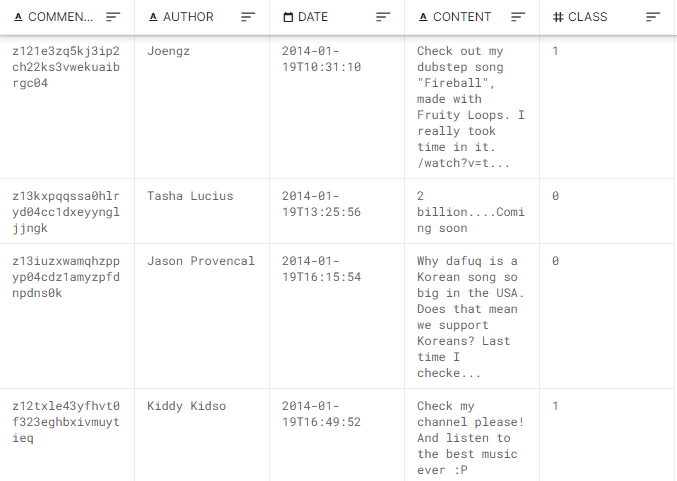
\includegraphics[width = 0.8\textwidth]{immagini/datasetExample.png}
        \caption{Immagine di uno dei dataset iniziali}

    \end{figure}


    E' stato scelto questo dataset in quanto i commenti susseguenti i video si avvicinavano alle possibili tuple di commenti
    di un reale caso applicativo all'interno della piattaforma.
    Inoltre presentava un'ampia gamma di istanze, così da permettere un buon addestramento dell'agente.
    I CSV di commenti sono stati trovati a questo indirizzo: \newline 
    \href{https://www.kaggle.com/datasets/lakshmi25npathi/images}{https://www.kaggle.com/datasets/lakshmi25npathi/images}.
    
    \section{Pulizia del dataset}
    Il dataset durante la fase di feature extraction, 
    è stato privato delle colonne: "COMMENT\textunderscore ID", "AUTHOR", "DATE", in quanto avrebbero potuto falsare i risultati dell'agente, 
    perchè non inerenti all'identificazione di un commento spam.
    L'operazione di pulizia si è poi composta delle seguenti fasi: 

    \begin{itemize}
        \item {\bfseries Conversione da uppercase a lowercase}, tutte le lettere in maiuscolo sono state convertite in minuscolo;
        \item {\bfseries Rimozione degli invii}, tutti i "break" sono stati rimossi;
        \item {\bfseries Rimozione della punteggiatura}, è stata eliminata ogni forma di punteggiatura;
        \item {\bfseries Rimozione dei link}, i commenti contenenti link ne sono stati privati;
        \item {\bfseries Rimozione degli spazi}, gli spazi consecutivi, ovvero in  quantità maggiore di 1, sono stati rimossi;
        \item {\bfseries Eliminazione lettere ripetute}, lettere identiche, ripetute in quantità maggiore di 2, sono state rimosse;
        \item {\bfseries Correzione delle parole}, parole non presenti all'interno del vocabolario inglese di Word Reference (scritte quindi in maniera errata oppure in tempi diversi dall'infinito), sono state sottoposte 
        ad un algoritmo di pattern matching. La funzione nello specifico, cerca inizialmente il match con parole di uso più comune. Nel caso in cui
        la parola presenti più matches, viene scelta la prima parola ad essere stata individuata;
        \item {\bfseries Eliminazione delle "stopwords"}, tutte le parole che rientravano nel dizionario delle stopwords (ovvero parole che non aggiungono alcuna informazione) 
        sono state eliminate;
        \item {\bfseries Rimozione valori nulli}, tutti i testi che, dopo aver superato questa scrematura, risultavano infine vuoti, sono stati eliminati. Si è scelto di effettuare direttamente la rimozione in quanto il dataset presentava un ampio numero di istanze.

 
    \end{itemize}
    \newpage
    
   

    \section{Bilanciamento del dataset}
    
    Il dataset, prima di poter essere sottoposto all'agente per l'addestramento, deve risultare bilanciato,
    altrimenti si rischia di incorrere in errate valutazioni da parte dell'agente (le minoranze risulterebbero sfavorite).
    \newline
    Il bilanciamento di un dataset si verifica quando il numero delle istanze appartenenti alle varie classi si equivale.
    Per verificare se il dataset preso d'esame risultasse bilanciato, sono state contate il numero di istanze appartenenti 
    alla classe "spam" e quelle appartenenti alla classe "ham", per ogni pezzo componente il dataset (ovvero le query di 
    commenti pubblicate sotto ogni videoclip) e successivamente sono state visualizzate su un grafico.
    
    \begin{figure}[h]
        \centering
        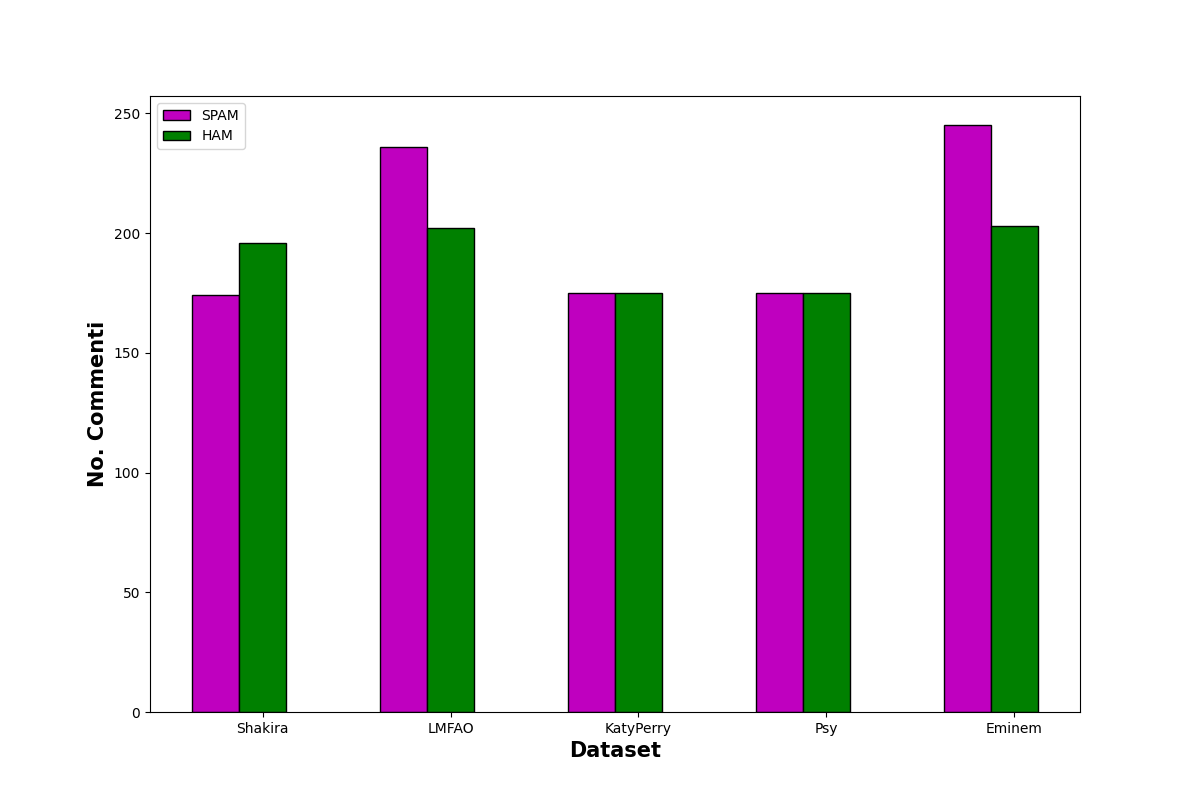
\includegraphics[width = \textwidth]{immagini/DatasetSeparati.png}
        \caption{Questo è il grafico della suddivisione fra spam ed ham nei vari dataset.}

    \end{figure}
    

   Nonostante per ogni videoclip, il numero di commenti spam ed ham tendevano ad equivalersi, si è preferito visualizzare
   anche la suddivisione del dataset nel suo totale.
    \newpage
    \begin{figure}[h!]
        \centering
        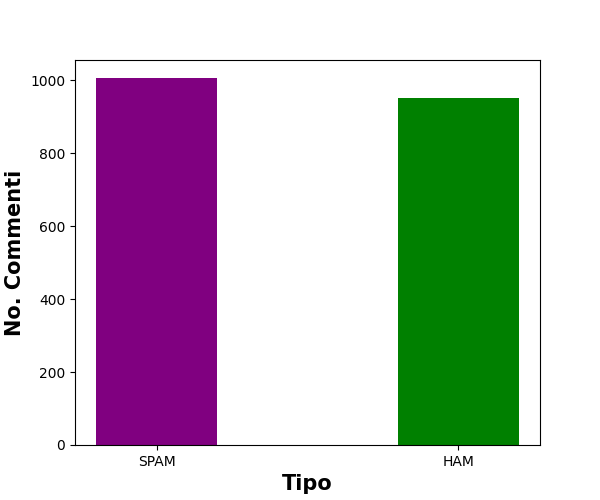
\includegraphics[height = 0.6\textwidth]{immagini/DatasetUnico.png}
        \caption{Questo è il grafico della suddivisione fra spam ed ham in tutti i dataset.}
    \end{figure}

    Si è quindi deciso di non procedere ad alcuna operazione di bilanciamento in quanto il dataset 
    risultava essere già di per se estremamente bilanciato.

    \chapter{Creazione agente}


    Dopo aver definito gli obiettivi dell'agente, le sue specifiche, l'ambiente in cui avrebbe lavorato ed il suo dataset, si è deciso come andava effettivamente costruito l'agente.
    Risulta evidente che, dovendo etichettare in una classe o nell’altra una certa istanza, il modello dell’agente debba essere scelto fra i classificatori. Dovendo stimare se un commento è un avviso pubblicitario o meno con il solo aiuto delle parole presenti nel commento, si è inizialmente individuata la frequenza con la quale ognuna di queste si presentava all’interno di ogni testo.
    In questo caso ci è venuta in aiuto la formula di Bayes:
    \newline
    \begin{equation}\label{bho}
        { p(B|A)  p(A)\over p(B)}
    \end{equation}
    \newline
    che, nel nostro caso, si traduce in:
    \newline
    \begin{equation}\label{bho2}
        p(spam|commento) = { p(commento|spam)  p(spam)\over p(commento)}
    \end{equation}
    \newline
    ovvero, la probabilità che un commento sia spam, è uguale alla probabilità che le parole del commento compaiano in un commento spam, dato che è spam, per la probabilità 
    che il commento sia spam, diviso la probabilità che queste parole compaiano nel commento.

    Si basano su questa formula tutta una famiglia di classificatori, detti classificatori "Naive Bayes" (Naive perchè assumono che ogni parola sia scritta in modo indipendente dalle altre).
    Si è deciso di concentrarsi su questa tipologia di algoritmi, effettuando diversi test per sceglierne il migliore.


    \section{Addestramento}
    Prima di poter addestrare l'agente, il dataset è stato sottoposto all'operazione di vettorizzazione, che consiste in due fasi:
    \begin{itemize}
        \item separazione del materiale testuale in un vettore contenente le singole parole (tokenizzazione);
        \item traduzione delle parole in numeri, rappresentanti la frequenza della parola all'interno del vettore iniziale.
    \end{itemize}
    A questo scopo è stata utilizzata la libreria "CounterVectorizer".
    \newline
    Una volta terminata questa fase, il dataset è stato suddiviso in 2 insiemi:
    \begin{itemize}
        \item {\bfseries Training Set}: la parte del dataset riservata all'addestramento dell'agente. E' stata costituita dal 
        70\% del dataset totale.
        \item {\bfseries Testing Set}: la parte del dataset riservata al testing dell'agente. Questo set di tuple è stato 
        costituito dal 30\% del dataset totale.
    \end{itemize}
    L'addestramento è stato effettuato su diversi tipi di classificatori, in modo da poter selezionare il migliore in fase di testing.
    I vari classificatori sono stati reperiti dalla libreria: \href{https://scikit-learn.org/stable/modules/naive_bayes.html}{https://scikit-learn.org/stable/modules/naive\textunderscore bayes.html}
    ed è stata utilizzata la versione 1.1.1.
    Nello specifico, ci si è concentrati principalmente su classificatori Naive Bayes in quanto la loro applicazione risulta consigliata
    su decisioni inerenti a brevi testi, in oltre risultano essere molto rapidi sia in fase di addestramento che in fase di esecuzione.
    Nello specifico sono stati messi a confronto i classificatori:
    \begin{itemize}
        \item {\bfseries GaussianNB}
        \item {\bfseries BernulliNB}
        \item {\bfseries ComplementNB}
        \item {\bfseries MultinomialNB}
    \end{itemize}

    \begin{figure}[h!]
        \centering
        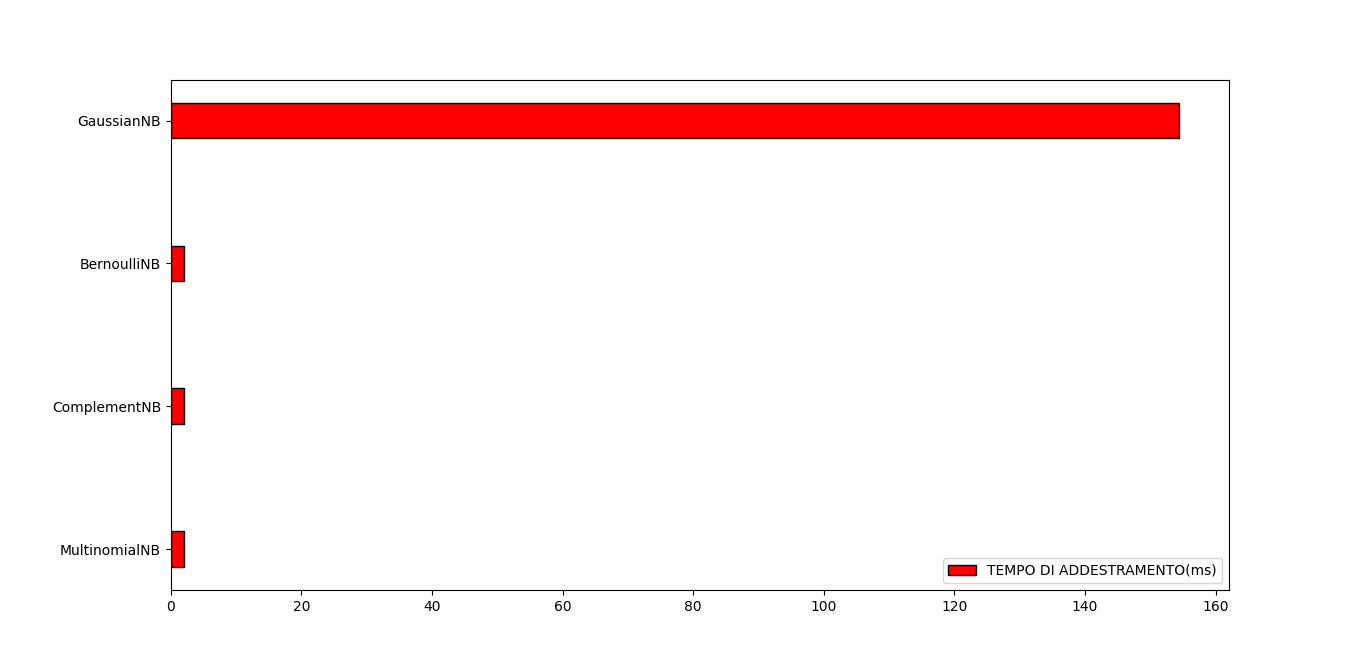
\includegraphics[width =\textwidth]{immagini/graficoAddestramento.png}
        \caption{Grafico che rappresenta i tempi di addestramento di diversi algoritmi Naive Bayes}

    \end{figure}

    In questa fase, il GaussianNB è risultato essere il più lento in fase di addestramento.


    
    
\newpage
    \section{Testing}
    Durante la fase di testing, i vari classificatori selezionati sono stati eseguiti sullo stesso Testing Set.
    I parametri che hanno influito nella scelta del classificatore da utilizzare sono stati:
    \begin{itemize}
        \item {\bfseries precision}, indica la quantità di previsioni corrette rispetto a tutte le istanze che ha classificato come spam;
        \item {\bfseries recall}, indica quante, fra tutte le istanze spam contenute nel Testing Set, sono state correttamente classificate come spam;
        \item {\bfseries accuracy}, indica il numero totale di previsioni giuste, fra spam ed ham;
        \item {\bfseries MCC}, è un coefficiente che si aggira fra 1 e -1. Questo intero rappresenta la media delle precisioni, dove per 1 
        si intende che il classificatore fa sempre la scelta giusta, mentre per -1 si intende che classifica sempre il contrario della realtà.  
    \end{itemize}

  
        \begin{figure}[h]
            \centering
            \includegraphics[width =\textwidth]{immagini/graficoBuono.png}
            \caption{Grafico che rappresenta vari parametri di diversi algoritmi Naive Bayes}

        \end{figure}
        
        Oltre ai parametri sopra elencati, è stato considerato anche il tempo di esecuzione.
        In questo caso il GaussianNB è risultato essere il più lento ad essere eseguito.
        \newpage
        
        \begin{figure}[h]
            \centering
            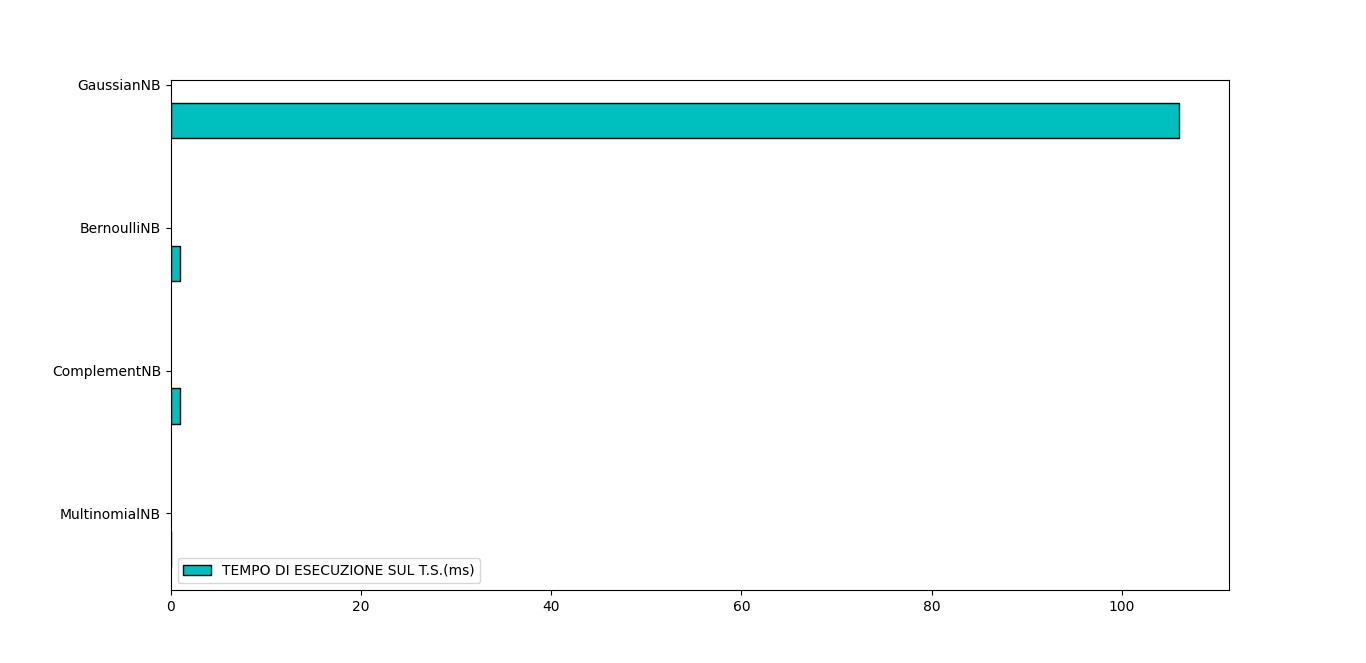
\includegraphics[width =\textwidth]{immagini/graficoEsecuzione.png}
            \caption{Grafico che rappresenta il tempo di esecuzione sul Testing Set di diversi algoritmi Naive Bayes}
        \end{figure}

    I vari test sono stati ripetuti anche modificando il Random State: il parametro che permette di ottenere un mescolamento e 
    una suddivisione tra training e testing set ripetibile nelle varie chiamate.
    Il valore ottimale del RandomState si è rivelato essere 42.
    

    \begin{figure}[h]
            \centering
            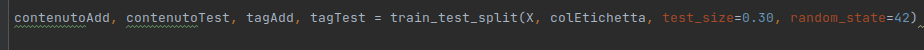
\includegraphics[width =\textwidth]{immagini/randomState.png}
            \caption{Immagine di come è stato modificato il Random State in modo da essere ottimizzato}

    \end{figure}

    In base ai vari parametri mostrati in precedenza, è stato scelto di adottare il ComplementNB come modello per l'agente.
   
    
    \section{Scelta del modello}
    Il ComplementNB è un tipo di algoritmo che si è dimostrato essere particolarmente preciso ed accurato.
    Come tutti i Naive Bayes si basa sulla formula di Bayes della probabilità condizionata.
  
    
    La sua particolarità consiste nel fatto che, al posto di calcolare e scegliere la maggiore probabilità 
    di appartenere ad una certa classe, calcola "il complemento" della probabilità di appartenere a tutte
    le classi (ovvero di non appartenervi) 
    
    \newline
    \textbf{Formula generale su cui si basa il Multinomial Naive Bayes}
    \begin{equation}
    \centering
        argmax \ p(y)*\Pi p(w|y)^fi
        \end{equation}
        
        \textbf{Formula specifica per il Complement Naive Bayes}
        \begin{equation}
        \centering
        argmin \ p(y)*\Pi\frac{1}{(w|\hat{y})^fi}
    \end{equation}
    \newline
    
    Più nel dettaglio:
    \begin{itemize}
        \item Calcola per ogni classe, data un'istanza, la probabilità di non appartenervi.
        \item Dopo aver calcolato questa probabilità per ogni classe, sceglie il più piccolo valore fra i risultati.
        \item Viene selezionato il valore più piccolo in quanto sarà la più piccola probabilità di {\bfseries NON APPARTENERE}
        a quella determinata classe, ovvero la più alta probabilità di appartenervi. Viene quindi selezionata quest'ultima.
    \end{itemize} 
    
    \chapter{Esecuzione agente}
    
    L'agente, per poter essere eseguito, deve essere integrato all'interno della piattaforma Storytelling.
    I due sistemi dovranno poter comunicare nonostante siano stati implementati in linguaggi diversi.
    \newline
    A questo scopo sono state utilizzate delle tecniche che, oltre a essere funzionali per la piattaforma in questione,
    renderanno più agevole l'integrazione dell'agente anche in altre piattaforme, scritte in qualsivoglia linguaggio.

    \section{Prelevamento istanze}
    Il sistema di comunicazione fra l'agente e la piattaforma, essendo scritte rispettivamente in Python 3.10 ed in Java 15.0.2, è stato 
    implementato tramite una socket, sulla quale l'agente ogni 24h:
    \begin{itemize}
        \item si avvia ad un orario prestabilito;
        \item rimane in attesa, fino alla ricezione della richiesta di Storytelling;
        \item riceve dalla socket la lista di commenti da analizzare, in formato JSON, assieme al loro corrispettivo autore;
        \item li inserisce in un dataframe generato tramite la libreria Pandas ed esegue le operazioni di pulizia, avviandole su processi differenti;
        \item esegue la classificazione;
        \item inoltra sulla socket i nominativi degli autori dei commenti che sono stati classificati come spam;
        \item chiude la socket e si termina la sua esecuzione;
    \end{itemize}

    \begin{figure}[h!]
        \centering
        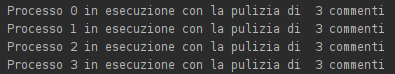
\includegraphics[width =0.5\textwidth]{immagini/puliziaCommenti.png}
        \caption{Avvio dei diversi processi di pulizia in parallelo}

    \end{figure}

    \begin{figure}[h!]
        \centering
        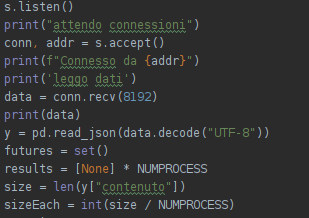
\includegraphics[width =0.4\textwidth]{immagini/socket.png}
        \caption{Immagine di come è stata implementata la comunicazione}

    \end{figure}

    \newpage
    \section{Risultati finali}
    L'agente, eseguito infine sulla piattaforma, è risultato avere una recall estremamente elevata, classificando
    correttamente le istanze spam, anche se peccando un pò di precision ed accuracy, presentando una leggera tendenza a 
    categorizzare come spam anche alcuni commenti che non lo erano.

    Eseguito sulle diverse occorrenze, si è però dimostrato estremamente attendibile, ed utilizzato nella quotidianità
    di un social svolgerebbe egregiamente il suo compito di supervisione.

    \begin{figure}[h!]
        \centering
        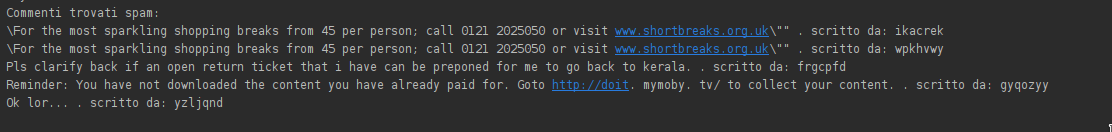
\includegraphics[width =\textwidth]{immagini/commentiSpam.png}
        \caption{Breve esempio di categorizzazione di alcuni commenti Spam}

\end{figure}




\end{document}
